\section{Overview}

The CLAS12 spectrometer in Hall~B at Jefferson Laboratory (JLab) has been designed and built for
comprehensive experimental studies of matter, using primarily a high-energy electron beam~\cite{clas12-nim}.
For these experiments this spectrometer must be capable of detecting scattered electrons within the entirety
of its forward acceptance range and at the highest possible efficiency with low background. The High
Threshold Cherenkov Counter (HTCC) (see Fig.~\ref{fig:Picture1}) of CLAS12 was designed and built to fulfill
the goal of detecting scattered electrons in the range of polar angles from 5$^\circ$ to 35$^\circ$ in
conjunction with other detector systems of the CLAS12 Forward Detector and to generate a fast trigger signal
for event readout.

\begin{figure}[ht]
    \centering
    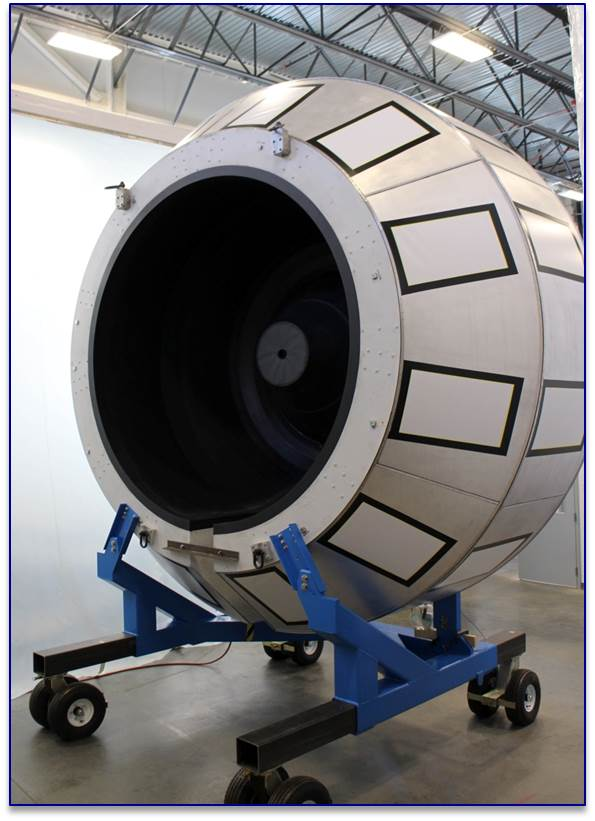
\includegraphics[width=0.75\linewidth]{images/Picture1.jpg}
    \caption{Fully assembled High Threshold Cherenkov Counter.}
    \label{fig:Picture1}
\end{figure}
The distinguishing features of the detector were influenced by its location in front of the drift chambers
(DC)~\cite{dc-nim}, which required that the HTCC incorporate a minimum amount of material in the active
area in front of the tracking detectors. Because the HTCC is a single module system, it occupies very limited
space within CLAS12. Consequently, the construction requirements (including transportation to the hall and
installation into the nominal location of the detector) were important for its structural design. 
